%!TEX root=../robocert.tex
\begin{figure}
	\centering
	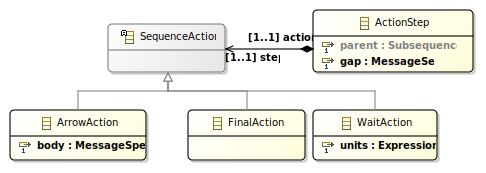
\includegraphics[width=0.7\textwidth]{diagrams/Actions}
	\caption{Class diagram for the part of the \langname{} metamodel dealing with actions.}
	\label{fig:metamodel-actions}
\end{figure}

\Cref{fig:metamodel-actions} depicts the part of the metamodel concerning
sequence actions.

A \msequenceaction{} is an explicit communication or control flow construct in a
\msubsequence.  There are currently three types of action: arrow, loop, and
final actions.

\subsection{\marrowaction}

An \marrowaction\footnote{The name signifies both that the actions resemble
PSC \emph{arrowMSG} specifications, and also that they correspond to arrows in
the graphical syntax.} specifies one communication between \mactor s which is on
the sequence specified by the diagram.  Each \marrowaction{} wraps one
\marrowmessagespec{} (\cref{sec:metamodel-messages})
containing the specification proper.
\todo{Eventually these will bind arguments.}

\begin{figure}[h!]
\begin{subfigure}[t]{\egtextwidth}
\begin{lstlisting}[style=Example]
-> operation O1()
\end{lstlisting}
\end{subfigure}
\hfill
\begin{subfigure}[t]{\eggraphicalwidth}
\gsecaption
\centering
\begin{tikzpicture}
\matrix[diagram]{
    \node[rcmodule](mstart) {\egtarget}; & \node[world](wstart) {\egworld}; \\
	\coordinate(mo); & \coordinate(wo); \\
	\coordinate(mend); & \coordinate(wend); \\
};
\draw[lifeline] (mstart) -- (mo) -- (mend);
\draw[lifeline] (wstart) -- (wo) -- (wend);
\draw (mo) edge[oarrow, "O1()"] (wo);
\end{tikzpicture}
\end{subfigure}

\end{figure}

\subsection{\mloopaction}

% Shorthand for introducing the loop action diagram matrix.
\newcommand{\egloopmatrix}{
  \node[rcmodule](mstart) {\egtarget}; \pgfmatrixnextcell \node[world](wstart) {\egworld}; \\
  \coordinate(mls); \pgfmatrixnextcell \coordinate(wls); \\
  \coordinate(mo); \pgfmatrixnextcell \coordinate(wo); \\
  \coordinate(mle); \pgfmatrixnextcell \coordinate(wle); \\
}
% Draws the entire loop diagram with the given loop bound header.
\newcommand{\egloopdiagram}[1]{
  \matrix[diagram]{\egloopmatrix};
  \draw[lifeline] (mstart) -- (mls) -- (mo) -- (mle);
  \draw[lifeline] (wstart) -- (wls) -- (wo) -- (wle);
  \draw (mo) edge[oarrow, "O1()"] (wo);
  \gloop{mls}{wls}{mle}{wle}{L}{#1}
}

A \mloopaction{} is a \emph{named} loop.  Each \mloopaction{} contains one
\msubsequence{} of steps to repeat indefinitely.

The number of times a \mloopaction{} will iterate \todo{breaking forthcoming}
depends on its attached \mloopbound{}.  Each bound is in terms of
\mexpression{}s that are evaluated \emph{only once}, before the execution
of the loop.

\paragraph{\minfiniteloopbound}
A \minfiniteloopbound{} states that the loop executes an infinite
number of times.

\begin{figure}[h!]
\begin{subfigure}[t]{\egtextwidth}
\begin{lstlisting}[style=Example]
loop L : forever { // or 'loop L {'
    -> operation O1()
}
\end{lstlisting}
\end{subfigure}
\hfill
\begin{subfigure}[t]{\eggraphicalwidth}
  \gsecaption
  \centering
  \begin{tikzpicture}
    \egloopdiagram{\gloopinfinite}
  \end{tikzpicture}
\end{subfigure}
\end{figure}

\paragraph{\mdefiniteloopbound}
A \mdefiniteloopbound{} states that the loop executes exactly the
number of times given in the bound.

\begin{figure}[h!]
\begin{subfigure}[t]{\egtextwidth}
\begin{lstlisting}[style=Example]
loop L : exactly 4 times {
    -> operation O1()
}
\end{lstlisting}
\end{subfigure}
\hfill
\begin{subfigure}[t]{\eggraphicalwidth}
  \gsecaption
  \centering
  \begin{tikzpicture}
    \egloopdiagram{\gloopdefinite{4}}
  \end{tikzpicture}
\end{subfigure}
\end{figure}

\paragraph{\mlowerloopbound}
A \mlowerloopbound{} states that the loop executes at least the
number of times given in the bound, but may nondeterministically
choose to execute any number of times in addition.

\begin{figure}[h!]
\begin{subfigure}[t]{\egtextwidth}
\begin{lstlisting}[style=Example]
loop L : at least 5 times {
    -> operation O1()
}
\end{lstlisting}
\end{subfigure}
\hfill
\begin{subfigure}[t]{\eggraphicalwidth}
  \gsecaption
  \centering
  \begin{tikzpicture}
    \egloopdiagram{\glooplower{5}}
  \end{tikzpicture}
\end{subfigure}
\end{figure}

\paragraph{\mrangeloopbound}
A \mrangeloopbound{} behaves as a \mlowerloopbound, but states that
the loop will not execute any more times than the given upper bound.
Note that if the bounds are the same, the semantics is equivalent
to that of a \mdefiniteloopbound{}.

\begin{figure}[h!]
\begin{subfigure}[t]{\egtextwidth}
\begin{lstlisting}[style=Example]
loop L : between 3 and 6 times {
    -> operation O1()
}
\end{lstlisting}
\end{subfigure}
\hfill
\begin{subfigure}[t]{\eggraphicalwidth}
  \gsecaption
  \centering
  \begin{tikzpicture}
    \egloopdiagram{\glooprange{3}{6}}
  \end{tikzpicture}
\end{subfigure}
\end{figure}

\subsection{\mfinalaction}

A \mfinalaction{} captures the successful termination of a sequence diagram.
A diagram with a \mfinalaction{} specifies a complete sequence of behaviour
from the \mtarget{} initialising to the \mtarget{} terminating.  Conversely,
sequence diagrams without \mfinalaction s capture partial specifications of
behaviour, or the behaviour of \mtarget s that do not terminate.

Note that the final \msequencegap{} before a \mfinalaction{} captures
any permitted communications after the behaviour explicitly specified by the
diagram has occurred.

\begin{figure}[h]

\begin{subfigure}[t]{\egtextwidth}
\begin{lstlisting}[style=Example]
end
\end{lstlisting}
\end{subfigure}
\hfill
\begin{subfigure}[t]{\eggraphicalwidth}
\gsecaption
\centering
\begin{tikzpicture}
\matrix[diagram]{
	\node[rcmodule](mstart) {\egtarget}; & \node[world](wstart) {\egworld}; \\
	\coordinate(mend); & \coordinate(wend); \\
};
\draw[lifeline] (mstart) -- (mend);
\draw[lifeline] (wstart) -- (wend);
\gfinal{mend}{wend}
\end{tikzpicture}
\end{subfigure}

\end{figure}

%%% Local Variables:
%%% mode: latex
%%% TeX-master: "../robocert"
%%% End:
